\documentclass[a4paper,11.5pt,table]{article}
\usepackage[textwidth=170mm, textheight=230mm, inner=20mm, top=20mm, bottom=30mm]{geometry}
\usepackage[normalem]{ulem}
\usepackage[utf8]{inputenc}
\usepackage[T1]{fontenc}
\PassOptionsToPackage{defaults=hu-min}{magyar.ldf}
\usepackage[magyar]{babel}
\usepackage{amsmath, amsthm,amssymb, paralist, tikz, multirow}
\usetikzlibrary{arrows, positioning}

\usepackage{listings}
\lstdefinestyle{customc}{
	belowcaptionskip=1\baselineskip,
	breaklines=true,
	frame=L,
	language=C++,
	showstringspaces=false,
	basicstyle=\ttfamily,
	%identifierstyle=\color{blue},
	keywordstyle=\bfseries\color{green!40!black},
	stringstyle=\color{orange},
	emph = {std, A, B, BDIT, Base, BaseOne, BaseTwo, C, CharT, Circle, Compr, ConstIterator, Cont, D, Deltoid, Derived, Derived2, DerivedLast, DerivedOne, DerivedTwo, detail, Fact, Fiu, Foo, Greater, Hallgato, IT, InputIt, Iterator, Kor, Lany, Less, LessByX, LinAlgVector, List, Matrix, Negyszog, Negyzet, RAIT, Rombusz, S, Sielo, Sikidom, StringLength, T, T1, T2, Templ, U, Val, X, Y, Z, bad_cast, bidirectional_iterator_tag, const_iterator, deque, forward_iterator_tag, input_iterator_tag, iostream, istream, iterator, iterator_category, line_editor, list, map, multimap, multiset, ostream, pair, random_access_iterator_tag, set, string, strlen, strlenWrong, value_type, vector}, 
	emphstyle = \color{blue},
	tabsize = 4
}

\lstdefinestyle{customasm}{
	belowcaptionskip=1\baselineskip,
	frame=L,
	language=[x86masm]Assembler,
	basicstyle=\ttfamily,
	commentstyle=\itshape\color{purple!40!black},
}

\lstset{
	escapechar=@,
	style=customc,
	literate =  {á}{{\'a}}1 {é}{{\'e}}1 {í}{{\'i}}1 {ó}{{\'o}}1 {ú}{{\'u}}1
	{Á}{{\'A}}1 {É}{{\'E}}1 {Í}{{\'I}}1 {Ó}{{\'O}}1 {Ú}{{\'U}}1
	{ö}{{\"o}}1 {ü}{{\"u}}1 {Ö}{{\"O}}1 {Ü}{{\"U}}1
	{ű}{{\H{u}}}1 {Ű}{{\H{U}}}1 {ő}{{\H{o}}}1 {Ő}{{\H{O}}}1
	{€}{{\euro}}1 {£}{{\pounds}}1	
}

\usepackage{hyperref}

\begin{document}
	%%%%%%%%%%%RÖVIDÍTÉSEK%%%%%%%%%%
	\setlength\parindent{0pt}
	\def\<{<\hspace{0mm}<}
	
	\theoremstyle{definition}
	\newtheorem{note}{Megjegyzés}[subsection]
	%%%%%%%%%%%%%%%%%%%%%%%%%%%%%%%%%%%%%%%%%%%%%%%%%%%%%%%%%%%%%%%%%%%%%
	
	\begin{center}
		{\LARGE\textbf{C++}}
		
		{\Large Gyakorlat jegyzet}
		
		7. óra.
	\end{center}
	A jegyzetet \textsc{Umann} Kristóf készítette \textsc{Horváth} Gábor gyakorlatán. (\today)
	\subsection{Header fájlra és fordításra egységre szétbontás}
	Ha egy darab header fájlban tárolnánk mindent, számos problémába ütköznénk. Ha több fordítási egységbe illesztenénk be a headert, fordítási idejű hibát kapnánk, hogy számos függvényt többször próbáltunk definiálni (sértenénk az ODR-t). Erre megoldás lehet, hogy a definíciókat és deklarációkat elválasztjuk: az osztályban lévő függvények deklarációit hagyjuk meg a header fájlban, és a definíciókat egy külön fordítási egységbe tegyük!
	
	\begin{note}
		Feltűnhet majd, hogy pár függvénydefiníció bent maradt. Erre később lesz magyarázat.
	\end{note}
	
	\medskip
	\fbox{\textbf{list.hpp:}}
\begin{lstlisting}
#ifndef LIST_H
#define LIST_H

#include <iosfwd>

class List;

class Iterator 
{
public:
	explicit Iterator(List *p) : p(p) {}
	bool operator==(Iterator other) const { return p == other.p; }
	bool operator!=(Iterator other) const { return !(*this == other); }
	Iterator operator++();
	int& operator*() const;
private:
	friend class ConstIterator;
	List *p;
};

class ConstIterator
{
public:
	ConstIterator(Iterator it) : p(it.p) {}
	explicit ConstIterator(const List *p) : p(p) {}
	bool operator==(ConstIterator other) const { return p == other.p; }
	bool operator!=(ConstIterator other) const { return !(*this == other); }
	ConstIterator operator++();
	int operator*() const;
private:
	const List *p;
};

class List 
{
public:
	explicit List(int data_, List *next = 0) : data(data_), next(next) {}
	~List() { delete next; }
	List(const List &other);
	List& operator=(const List &other);
	void add(int data);
	Iterator begin() { return Iterator(this); }
	ConstIterator begin() const { return ConstIterator(this); }
	Iterator end() { return Iterator(0); }
	ConstIterator end() const { return ConstIterator(0); }
private:
	friend Iterator;
	friend ConstIterator;
	int data;
	List *next;
};

#endif
\end{lstlisting}

	\fbox{\textbf{list.cpp:}}
\begin{lstlisting}
#include <iostream>

#include "list.hpp"
#include <iostream>

List::List(const List &other) : data(other.data), next(0) 
{
	if (other.next != 0) 
	{
		next = new List(*other.next);
	}
}

List& List::operator=(const List &other) 
{
	if (this == &other)
		return *this;
	delete next;
	data = other.data;
	if (other.next) 
	{
		next = new List(*other.next);
	} 
	else 
	{
		next = 0;
	}
	return *this;
}

void List::add(int data) 
{
	if (next == 0) 
	{
		next = new List(data);
	} 
	else 
	{
		next->add(data);
	}
}

Iterator Iterator::operator++() 
{
	p = p->next;
	return *this;
}

int& Iterator::operator*() const 
{
	return p->data;
}

ConstIterator ConstIterator::operator++() 
{
	p = p->next;
	return *this;
}

int ConstIterator::operator*() const 
{
	return p->data;
}
\end{lstlisting}
	\fbox{\textbf{main.cpp:}}
\begin{lstlisting}
#include <iostream>
#include "list.hpp"

void print(const List &l)
{
	for(ConstIterator it = l.begin(); it != begin(); ++it)
	{
		std::cout << *i << ' ';
	}
	std::cout << std::endl;
}

int main() 
{
	List head(5);
	head.add(8);
	head.add(10);
	head.add(8);
}

\end{lstlisting}
	
	Ez a szétválasztás sok egyéb előnnyel is jár: a \texttt{List}-hez tartozó információk sokkal kisebb helyen elférnek. Azonban ahogy a fenti megjegyzés is felhívta rá a figyelmet, a list.hpp továbbá is tartalmaz definíciókat! Ennek ellenére azt tapasztaljuk, hogyha több fordítási egységbe illesztjük be a headert, még akkor sem kapunk fordítási idejű hibát. Ennek a magyarázatához tegyünk egy kisebb kitérőt.
	\subsection{Inline függvények}
	
	Tekintsük azt a példát, amikor a \texttt{void f() \{\}} függvényt is beillesztjük a headerbe: ha több fordítási egységet fordítanánk egyszerre, melybe ez a header be van illesztve, linkelési hibát kapnánk, mert \texttt{f} többször lesz definiálva. Ez azonban megkerülhető az \texttt{inline} kulcsszó használatával, segítségével ugyanis kiküszöbölhető a linker hiba: minden azonos nevű, visszatérési értékű, és paraméter listájú inline-ként definiált függvény definícióval együtt beilleszthető több különböző fordítási egységbe, és nem fog fordítási hibát okozni.
	
	Ez úgy oldható meg, hogy a fordító a linkelés folyamán a definíciók közül egyet tetszőlegesen kiválasztást. Az osztályon belül kifejtett függvények implicit inline-ok, így sose okozhatnak fordítási hibát.
	\begin{lstlisting}
inline void f() {}
	\end{lstlisting}
	Az ábra jól demonstrálja a problémát.
	\begin{figure}[h]
		\centering
		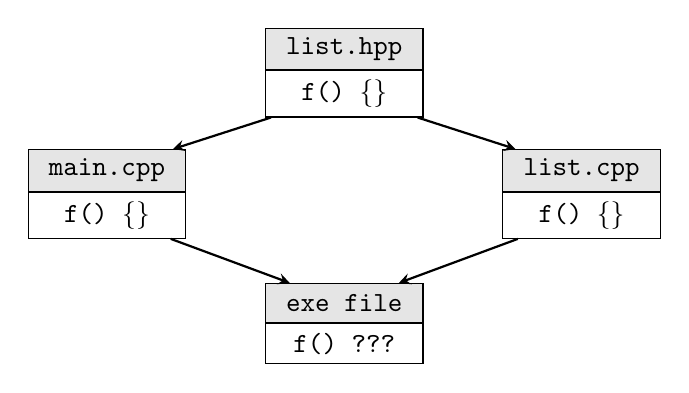
\begin{tikzpicture}
		\tikzstyle{HeaderName} = [rectangle, minimum width=2cm, minimum height=5mm, text centered, draw=black, fill= gray!20]
		\tikzstyle{CppName} = [rectangle, minimum width=2cm, minimum height=5mm, text centered, draw=black, fill= gray!20]
		\tikzstyle{FunctionName} = [rectangle, minimum width=2cm, minimum height=5mm, text centered, draw=black, fill= white]
		\tikzstyle{arrow} = [thick,->,>=stealth]
		
		
		\node (listHpp) [HeaderName] {\texttt{list.hpp}};
		\node (listHppF) [FunctionName, below = 0 mm of listHpp] {\texttt{f() \{\}}};
		
		\node (mainCpp) [CppName, below left = of listHpp] {\texttt{main.cpp}};
		\node (mainCppF) [FunctionName, below  = 0 mm of mainCpp] {\texttt{f() \{\}}};
		
		\node (listCpp) [CppName, below right = of listHpp] {\texttt{list.cpp}};
		\node (listCppF) [FunctionName, below  = 0 mm of listCpp] {\texttt{f() \{\}}};
		
		\node (exe) [CppName, below = 2.7 cm of listHpp] {\texttt{exe file}};
		\node (exeF) [FunctionName, below  = 0 mm of exe] {\texttt{f() ???}};
		
		\draw[arrow] (listHppF) -- (mainCpp);
		\draw[arrow] (listHppF) -- (listCpp);
		\draw[arrow] (mainCppF) -- (exe);
		\draw[arrow] (listCppF) -- (exe);
		\end{tikzpicture}
		\smallskip
		
		A \texttt{main.cpp}-ben vagy a \texttt{list.cpp}-ben lévő definíciója szerepeljen \texttt{f}-nek a futtatható fájlban?
	\end{figure}
	\texttt{f()} egy un. \textit{strong reference}-el jön létre ha nem inline, így a linker hibát dob ha több fordítási egységben definiálva van. Ha azonban inline-ként adjuk meg, akkor  \textit{weak reference}-ként értelmezi, a meglevő definíciók közül tetszőlegesen kerül egy kiválasztásra. Ez nyilván azt is jelenti, hogy minden ilyen függvény definíciójának meg kell egyeznie, hisz kellemetlen meglepetés érhet minket, ha különböző definíciók közül olyat választ a fordító, melyre nem számítanánk (és ez egyben nem definiált viselkedés is).
	\begin{note}
		A legtöbb fordítónál lehet egy LTO (\textit{link time optimalization}) funkciót bekapcsolni, mely a linkelésnél optimalizál, többek között ott végzi el az inlineolást.
	\end{note}
	\begin{note}
		Az inline függvények hajlamosak erősen megnövelni a bináris kódot, így az erőltetett használatuk nem javallott.
	\end{note}
	\begin{note}
		Az inline kulcsszó egy javaslat a fordítónak, de nem parancs. Nem inline függvények lehetnek inline-ok, és inlineként definiált függvények lehet mégsem lesznek azok.
	\end{note}
	Azok a tagfüggvények, melyek nem az osztály törzsében vannak definiálva, nem lesznek inline-ok, ezért volt az, hogy mielőtt szétszedtük a listánkat header fájlra és fordítási egységre, linkelési hibát kaptunk (\texttt{Iterator} és \texttt{ConstIterator} pár tagfüggvénye külön volt véve).
	\medskip
	
	Cseréljük le a print függvényt:
	%TODO nem ártana megmagyarázni, ez miért nem tagfüggvény
	\begin{lstlisting}
std::ostream& operator<<(std::ostream &os, const List &l)
{
	for(ConstIterator it = l.begin(); it != l.end(); ++it)
	{
		os << *it;
	}
	return os;
}
	\end{lstlisting}
	Sajnos ismét fordítási hibát kapunk, hisz a fordító nem tudja mi az az \texttt{ostream}, hisz az ismerős \texttt{iostream} könyvtár nincs include-olva. Ilyenkor azonban érdemes inkább az \texttt{iosfwd} headert beilleszteni az \texttt{iostream} helyett, mert ez minden beolvasással és kiíratással kapcsolatos osztály/függvénynek csak a deklarációját tartalmazza, és így csökken a fordítási egység mérete (azonban a cpp fájlban muszáj \texttt{iostream}-et használni, hogy a definíciók meglegyenek).
	\begin{note}
		Ha szeretnénk egy \texttt{std::ostream} típusú objektumot használni, szükségünk lenne az \texttt{iostream} könyvtárra, hisz a fordítónak tudnia kéne, mekkora az \texttt{std::ostream} mérete, és ehhez szüksége van a teljes osztálydefinícióra. Azonban a referencia vagy pointer típusoknál erre nincs szükség, amíg nem akarunk egy tagfüggvényüket meghívni.
	\end{note}
	\section{Névterek}
	A kódunkkal kapcsolatban felmerülhet egy másik probléma is: nagyon sok hasznos nevet elhasználtunk, pl. több \texttt{Iterator} nevű osztályt nem hozhatunk létre (az un. globális névtérbe vagy \textit{global namespace}-be kerültek), különben a névütközés áldozatai leszünk. Pedig várhatóan nem csak ennek az egy konténernek szeretnék iterátort írni.
	\smallskip
	
	Megoldás lehet, hogyha inline class-t hozunk létre, azaz az iterátor teljes deklarációját beillesztjük a \texttt{List}-be, így csak a \texttt{List} lát rá \texttt{Iterator}-ra követlenül, mindenhol máshol úgy kell hivatkozni rá, hogy \texttt{List::Iterator}.
	\begin{lstlisting}
class List
{
public:
	class Iterator
	{
		//...
	};
	//...
};
	\end{lstlisting}
	
	Azonban szerencsésebb, ha az iterátorainkat egy névtérbe (\textit{namesspace}) rakjuk.
\begin{lstlisting}
namespace detail
{
	class Iterator
	{
		//...
	};
	class ConstIterator
	{
		//...
	};
}
\end{lstlisting}
	Így az \texttt{Iterator} és \texttt{ConstIterator} osztályra a későbbiekben csak úgy hivatkozhatunk, ha megmondjuk, mely névtérből származnak. Ugyanezzel a módszerrel, ha létrehozunk pl. egy \texttt{Vector} nevű osztályt, annak is írhatunk egy \texttt{Iterator} nevű osztályt, amit pl. egy \texttt{VectorDetail} névtérbe tehetünk.
	\begin{lstlisting}
detail::Iterator it;
detail::ConstIterator cit;
	\end{lstlisting}

	A névterek segíthetnek abban, hogy logikai egységebre rendezzük a kódunkat. Az egyik legnagyobb ilyen egység az \texttt{std} névtér, mely tartalmaz minden függvényt, változót, stb, ami a standard részét alkotja. 
	
	Lehet névtereket egymásba is ágyazni, erre lehet példa a C++11-es \texttt{chrono} könyvtár, mely az \texttt{std} névteren belül számos dolgot a \texttt{chrono} alnévtérben tárol.
	\subsection{Argument Dependent Lookup}
	A szokásos Hello World programban nem feltétlenül kell használni a \texttt{using namespace std;} sort. Azonban megállapítható, hogy a \texttt{\<} operátor globális, \texttt{std} névtérbeli, mégse kellett elé \texttt{std} névtérre hivatkozás (azaz \textit{explicit namespace resolution}). Ez az úgynevezett ADL-nek (\textit{Argument Dependent Lookup}) köszönhető, melyet a fordító alkalmaz: az adott függvényt abban a névtérben keresi először, ahol az argumentumai megtalálhatóak.
	
	\smallskip
	Példaképp, a Hello World programban a \texttt{cout} változó az \texttt{std} névtér tagja, így a fordító először az \texttt{std} névtérben fogja keresni a \texttt{\<} operátort.
	\section{Typedef}
	A \texttt{typedef} kulcsszó szinonimák létrehozására használatos, és ha ügyesen használjuk, ki lehet használni valamennyi előnyét. 
	
	\smallskip
	Hozzunk létre egy osztályt, melynek adatokat kell tárolnia. Tegyük fel, hogy egyenlőre nem fontos számunkra az, hogy milyen konténerben tároljuk az adatokat az osztályon belül, és a példa kedvéért követeljük meg ettől a leendő konténertől hogy rendelkezzen \texttt{push\_back} tagfüggvénnyel. Az \texttt{std::vector} konténerrel ez így nézhetne ki:
	\begin{lstlisting}
class StoreIntData
{
private:
	std::vector<int> data;
};
	\end{lstlisting}
	Írjunk egy tagfüggvényt, mellyel két \texttt{StoreIntData} típus tárolt adatait össze tudjuk fűzni.
	\begin{lstlisting}
class StoreIntData
{
public:
	std::vector<int> merge(StoreIntData &other)
	{
		std::vector<int> ret;
		for(int i = 0; i<data.size(); i++)  ret.push_back(data[i]);
		for(int i = 0; i<other.size(); i++) ret.push_back(other.data[i]);
		return ret;
	}
private:
	std::vector<int> data;
};
	\end{lstlisting}
	\begin{note}
		Később látunk majd példát egy ennél jóval elegánsabb megoldásra is.
	\end{note}
	Tegyük fel, hogy az implementáció egy pontján úgy döntünk, mégse \texttt{std::vector}-ban, hanem \texttt{std::deque}-ban szeretnénk tárolni (erről a konténerről részletesen szó lesz később, egyenlőre legyen elég annyi, hogy az \texttt{std::vector}-hoz hasonló). Ekkor rákényszerülünk arra, hogy minden helyen, ahova \texttt{std::vector}-t írtunk, módosítanunk kelljen, és a kódismétlés áldozatai lettünk. Ehelyett használjunk egy \texttt{typedef}-et!
	\begin{lstlisting}
class StoreIntData
{
public:
	typedef std::deque<int> Container;
	
	Container merge(StoreIntData &other)
	{
		Container ret;
		for(int i = 0; i<data.size(); i++)  ret.push_back(data[i]);
		for(int i = 0; i<other.size(); i++) ret.push_back(other.data[i]);
		return ret;
	}
private:
	Container data;
};
	\end{lstlisting}
	Így ha módosítanunk kell a konténerünk típusát, elég a typedefet átírni.
	\medskip
	
	Visszatérve a láncolt listánkra, a módosítás után \texttt{List} nem tudja, mi az az \texttt{Iterator}, hisz az egy \texttt{datail} nevű névtérben van, ezért vagy minden \texttt{Iterator}-t lecserélünk \texttt{detail::Iterator}-ra, vagy pedig létrehozunk egy szinonimát.
	\begin{lstlisting}
class List
{
public:
	typedef detail::Iterator Iterator;
	typedef detail::ConstIterator ConstIterator;
	//...
};
	\end{lstlisting}
	A typedef segítségével viszont még egy dolgot nyertünk: mivel ezen a szinonimák publikusak, így az osztályon kívül is tudunk rájuk hivatkozni így:
	\begin{lstlisting}
List::Iterator it = head.begin();
	\end{lstlisting}
	
	
\end{document}
